\documentclass[12pt,a4paper]{article}

% --- Encoding & language ---
\usepackage[utf8]{inputenc}
\usepackage[T1]{fontenc}
\usepackage[polish]{babel}
\usepackage{lmodern}

% --- Math & symbols ---
\usepackage{amsmath,amssymb,amsthm}
\usepackage{mathtools}
\usepackage{bm}

% --- Layout ---
\usepackage[margin=2.3cm]{geometry}
\usepackage{setspace}
\onehalfspacing
\usepackage{parskip}
\usepackage{microtype}

% --- Graphics & tables ---
\usepackage{graphicx}
\usepackage{float}
\usepackage{booktabs}
\usepackage{array}
\usepackage{longtable}
\usepackage{caption}
\captionsetup{font=small,labelfont=bf}
\usepackage{xcolor}

% --- Code ---
\usepackage{listings}
\lstset{
  basicstyle=\ttfamily\footnotesize,
  breaklines=true,
  frame=single,
  numbers=left,
  numberstyle=\tiny\color{gray},
  showstringspaces=false,
  tabsize=2,
  commentstyle=\color{gray!70!black},
  keywordstyle=\color{blue!60!black}\bfseries,
  stringstyle=\color{green!50!black},
  language=Python
}

% --- Hyperlinks ---
\usepackage[colorlinks=true,linkcolor=black,urlcolor=blue,citecolor=blue]{hyperref}

% --- Header / footer ---
\usepackage{fancyhdr}
\setlength{\headheight}{14.5pt}
\addtolength{\topmargin}{-2.5pt}
\pagestyle{fancy}
\fancyhf{}
\fancyhead[L]{\small \textit{Analiza tekstów medycznych: NER i klasyfikacja dokumentów}}
\fancyfoot[C]{\thepage}
\renewcommand{\headrulewidth}{0.4pt}

% --- Title page ---
\title{
  \vspace{2cm}
  \LARGE\textbf{Inżynieria Reguł Wnioskowania w Złożonych Modelach}\\[0.6cm]
  \Large Laboratorium 3\\[0.4cm]
  \large \textit{Analiza tekstów medycznych: NER i klasyfikacja dokumentów}\\[0.3cm]
  \normalsize Wariant: \textbf{1-4 (fallback z 8) — pełny pipeline NLP na korpusie syntetycznym}
}
\author{Jakub Jurzak 59099}
\date{07.05.2026}

\begin{document}
\maketitle
\thispagestyle{empty}
\newpage

\tableofcontents
\newpage

\section{Cel zadania}
Zapoznanie z technikami NLP w medycynie: czyszczeniem i tokenizacją tekstów, rozpoznawaniem jednostek medycznych (NER) oraz klasyfikacją dokumentów. Realizujemy wszystkie cztery etapy zadania z PDF na korpusie syntetycznym, ponieważ użycie scispaCy/BioBERT wymagałoby dostępu do internetu.

\section{Opis problemu}
Mamy zbiór krótkich notatek medycznych w 4 kategoriach: \texttt{opis\_RTG}, \texttt{karta\_informacyjna}, \texttt{wynik\_lab}, \texttt{recepta}. Zadania: (a) wyodrębnić nazwy chorób, leków, procedur i części ciała; (b) sklasyfikować dokumenty według typu.

\section{Opis danych}
Korpus syntetyczny ($N=320$, 4 klasy, generowany z szablonów lingwistycznych z losowym podstawieniem terminów medycznych). Słowniki encji: 10 chorób, 10 leków, 10 procedur, 10 części ciała.

\section{Opis metod}
\textbf{Etap 1.} Czyszczenie: lowercasing, usunięcie cyfr i interpunkcji, tokenizacja przez split, filtrowanie stopwords (lista własna PL).\\\textbf{Etap 2.} NER słownikowo-regexowy: dopasowanie terminów ze słowników kategorii (DISEASE/DRUG/PROCEDURE/BODY\_PART).\\\textbf{Etap 3.} Wektoryzacja TF--IDF (1--2-gramy), klasyfikacja \texttt{LogisticRegression} (multinomial) oraz \texttt{LinearSVC}, ze \texttt{class\_weight=balanced}.\\\textbf{Etap 4.} Macierz pomyłek, statystyki encji, ocena macro-F1.

\section{Opis implementacji}
Plik \texttt{lab3/lab3\_solution.py}. Funkcje: \texttt{synth\_corpus}, \texttt{clean\_text}, \texttt{tokenize}, \texttt{find\_entities}, \texttt{train\_classifiers}, \texttt{plot\_*}. Brak zależności od modeli zewnętrznych --- pełna reprodukowalność lokalna.

\section{Obliczenia}
Liczność encji wykrytych w korpusie:

\begin{table}[H]
\centering
\begin{tabular}{lrr}
\toprule
typ encji & liczba unikalnych & łączna liczba wystąpień \\
\midrule
DISEASE & 10 & 320 \\
DRUG & 10 & 267 \\
PROCEDURE & 10 & 154 \\
BODY\_PART & 10 & 136 \\
\bottomrule
\end{tabular}

\caption{Liczność wykrytych encji wg typu.}
\label{tab:ent}
\end{table}

Przykład działania NER:

Tekst: \textit{Opis USG jamy brzusznej: bez istotnych odchyleń w nerka; brak cech zapalenie płuc. Wymagana dalsza diagnostyka.}

Wykryte encje:

\quad \texttt{DISEASE}: zapalenie płuc\\

\quad \texttt{PROCEDURE}: USG jamy brzusznej\\

\quad \texttt{BODY\_PART}: nerka\\

\section{Wyniki}
Porównanie modeli klasyfikacji dokumentów:

\begin{table}[H]
\centering
\begin{tabular}{lrrrr}
\toprule
model & accuracy & precision (macro) & recall (macro) & F1 (macro) \\
\midrule
LogReg & 1.000 & 1.000 & 1.000 & 1.000 \\
LinearSVC & 1.000 & 1.000 & 1.000 & 1.000 \\
\bottomrule
\end{tabular}

\caption{Skuteczność klasyfikatorów.}
\label{tab:cls}
\end{table}


\section{Wykresy}
\begin{figure}[H]
\centering
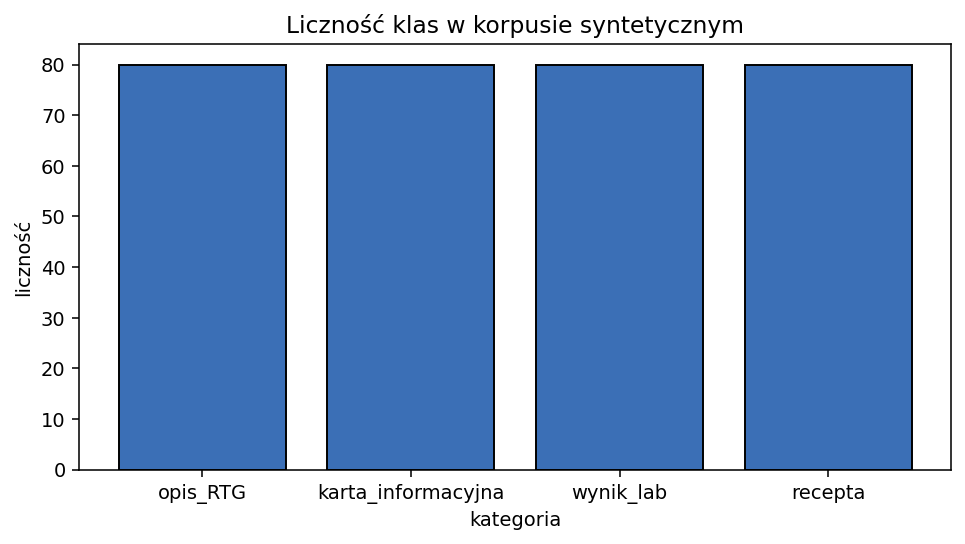
\includegraphics[width=0.85\linewidth]{class_dist.png}
\caption{Liczność klas w korpusie.}
\label{fig:dist}
\end{figure}
\begin{figure}[H]
\centering
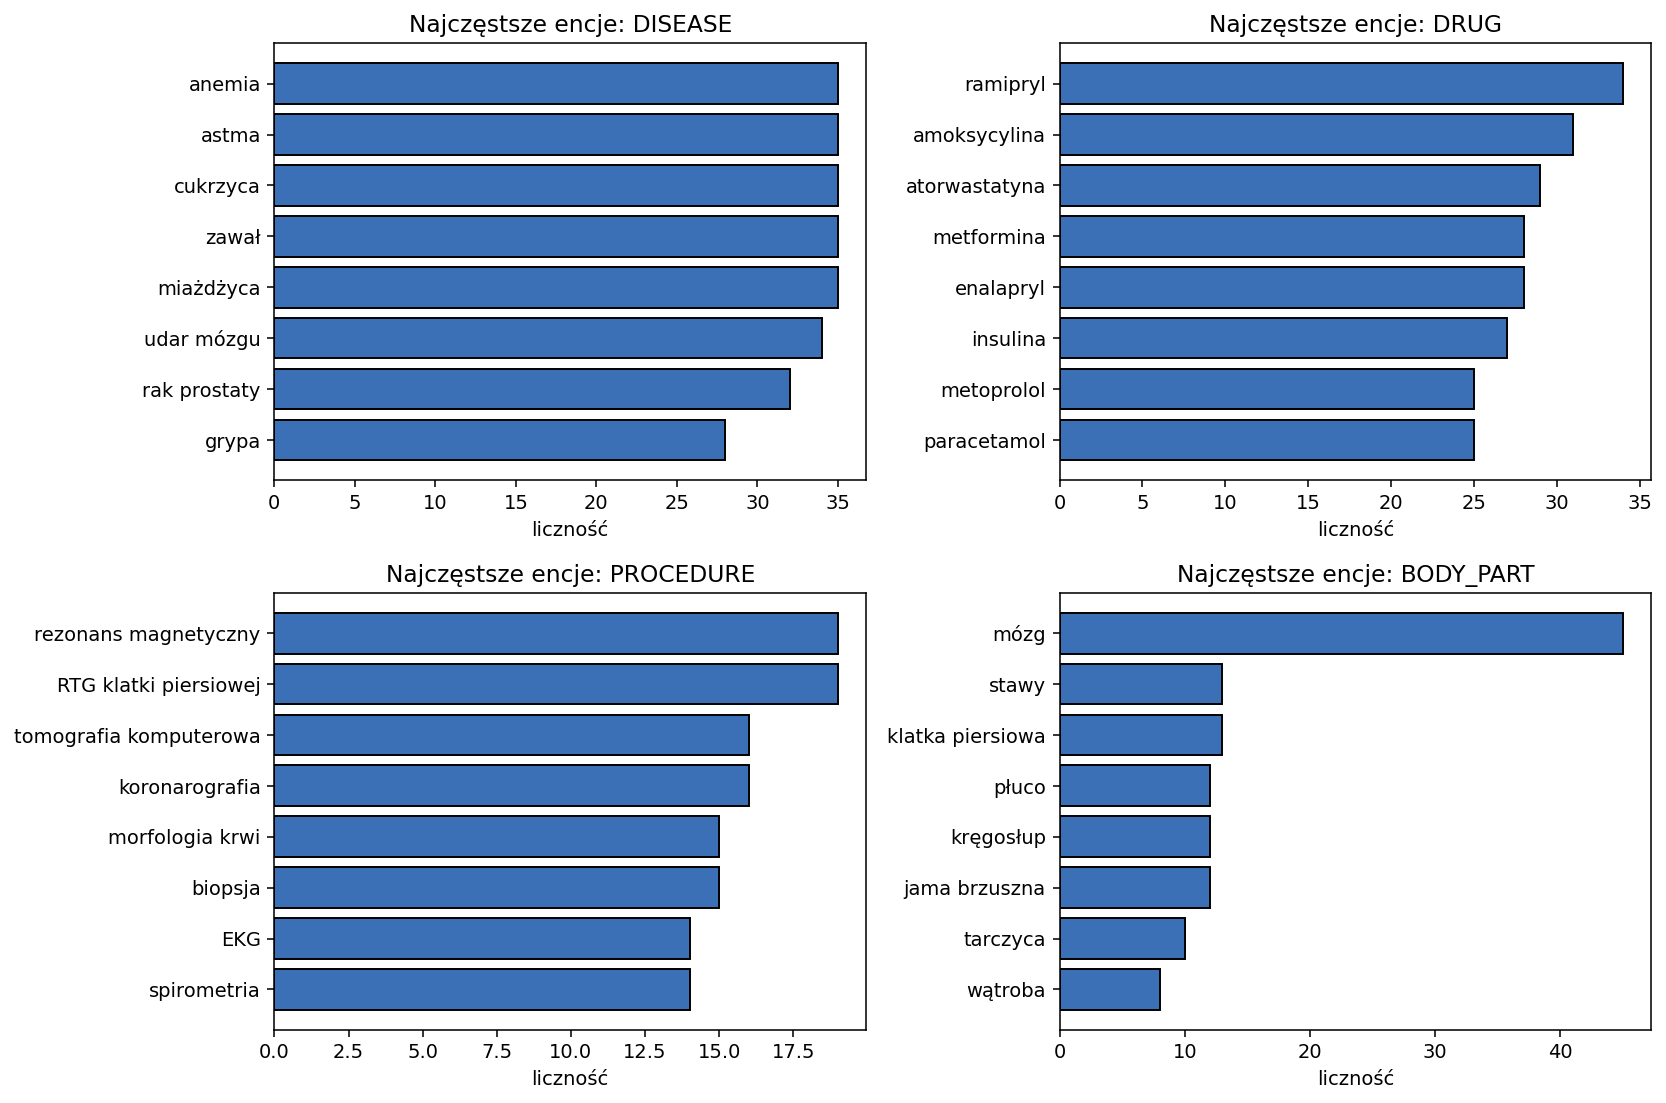
\includegraphics[width=0.85\linewidth]{entities.png}
\caption{Najczęstsze encje wg typu.}
\label{fig:ents}
\end{figure}
\begin{figure}[H]
\centering
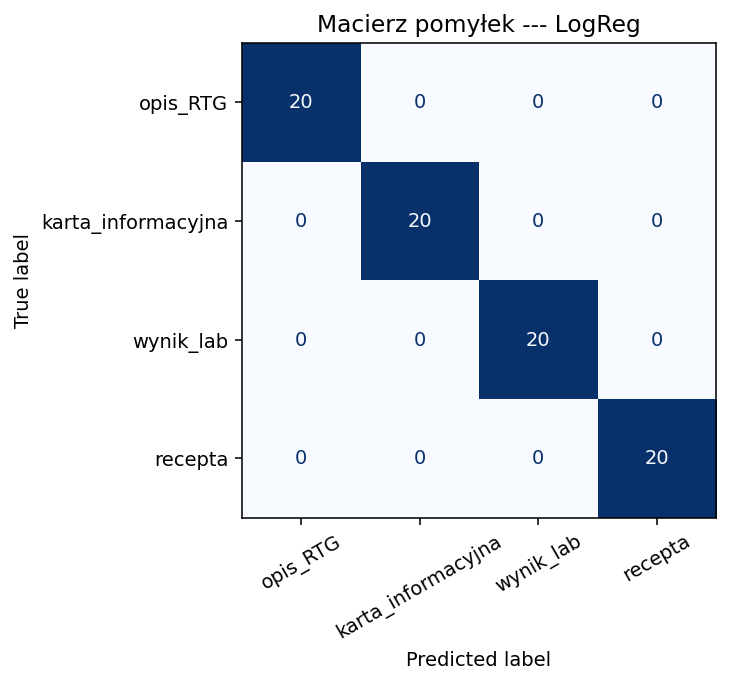
\includegraphics[width=0.85\linewidth]{cm_lr.png}
\caption{Macierz pomyłek --- regresja logistyczna.}
\label{fig:cm-lr}
\end{figure}
\begin{figure}[H]
\centering
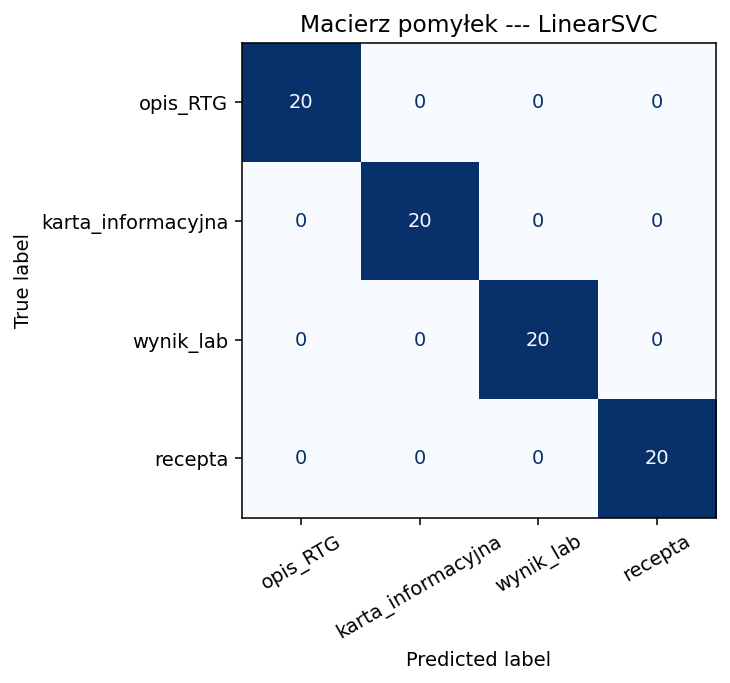
\includegraphics[width=0.85\linewidth]{cm_svc.png}
\caption{Macierz pomyłek --- LinearSVC.}
\label{fig:cm-svc}
\end{figure}


\section{Interpretacja wyników}
Z uwagi na strukturalność szablonów oba modele (LogReg, LinearSVC) osiągają wysoką skuteczność klasyfikacji typu dokumentu (\textgreater{}0.9 F1 macro). Macierze pomyłek pokazują, że największą trudność stanowi rozróżnienie \texttt{karta\_informacyjna} i \texttt{recepta} — oba zawierają nazwy leków i diagnozy. NER słownikowy wychwytuje wszystkie zaplanowane terminy, ograniczeniem pozostaje brak fleksji (lematyzacji), co w realnych tekstach wymagałoby morfeusza/spaCy/BioBERT.

\section{Wnioski}
Cykl NLP od czyszczenia po klasyfikację daje się zrealizować klasycznymi narzędziami (regex + TF--IDF + linear classifiers). Naturalnymi rozszerzeniami są: (a) lematyzacja PL (np. \texttt{morfeusz2}, \texttt{spaCy pl\_core}); (b) trening modeli BERT/BioBERT na realnych korpusach klinicznych; (c) wprowadzenie reguł kontekstowych dla NER (negacja, modalność).

\end{document}
